\documentclass[12pt,a4paper]{report}

\usepackage[cm]{fullpage}
\usepackage{paralist}
\usepackage{pdfpages}
\usepackage{graphicx}
\usepackage{wrapfig}
\usepackage{scrextend}
\usepackage[nottoc,chapter]{tocbibind}
\newcommand{\HRule}{\rule{\linewidth}{0.5mm}}
\title{Workflow thing}

\author{Michiel Johan Baird \\
        Department of Computer Science \\
        University of Cape Town
    \\   \small{Supervisor: Dr. Hussein Suleman} }

\begin{document}
\begin{titlepage}

\begin{center}


% Upper part of the page
\includegraphics[width=0.15\textwidth]{./images/cslogo}\\[1cm]


\textsc{\Large Honours Project Report}\\[0.5cm]


% Title
\HRule \\[0.4cm]
{ \huge \bfseries Proposed Workflow System that meets the requirements of the Zamani Project}\\[0.4cm]

\HRule \\[1.5cm]

% Author and supervisor
\begin{minipage}{0.4\textwidth}
\begin{flushleft} \large
\emph{Author:}\\
Michiel Johan \textsc{Baird}
\end{flushleft}
\end{minipage}
\begin{minipage}{0.4\textwidth}
\begin{flushright} \large
\emph{Supervisor:} \\
Dr.~Hussein \textsc{Suleman}
\end{flushright}
\end{minipage}

% Bottom of the page
\vfill
\begin{table}[h]
\centering
\begin{tabular}{|l|p{7.5cm}|l|l|l|}
\hline
& \textbf{Category} & \textbf{Min} & \textbf{Max} & \textbf{Chosen} \\
\hline
1 & Requirements Analysis and Design & 0 & 20 & 15 \\
\hline
2 & Theoretical Analysis & 0 & 25 & 0 \\
\hline
3 & Experiment Design and Execution & 0 & 20 & 10 \\
\hline
4 & System Development and Implementation & 0 & 15 & 10 \\
\hline
5 & Results Findings and Conclusion & 10 & 20 & 10 \\
\hline
6 & Aim Formulation and Background Work & 10 & 15 & 10 \\
\hline
7 & Quality of Report Writing and Presentation &
\multicolumn{2}{|c|}{10}  & 10 \\
\hline
8 & Adherence to Project Proposal and Quality of Deliverables &
\multicolumn{2}{|c|}{10}  & 10 \\
\hline
9 & Overall General Project Evaluation & 0 & 10 & 5 \\
\hline
\multicolumn{2}{|l|}{\textbf{Total}} & \multicolumn{2}{|l|}{\textbf{80}} & \textbf{80} \\
\hline
\end{tabular}
\end{table}




\textsc{\Large University of Cape Town}\\[0.5cm]
\textsc{\Large Department of Computer Science}\\[0.5cm]
{\large \today} \\
\end{center}
\HRule \\[0.2cm]
{\raggedleft The financial assistance of the National Research Foundation (NRF) towards this research is hereby acknowledged. Opinions
expressed and conclusions arrived at, are those of the author and are not necessarily to be attributed to the NRF.}\\
\HRule \\[0.2cm]



\end{titlepage}

\pagenumbering{roman}
\tableofcontents
\newpage
\listoffigures
\newpage
\begin{abstract}

\end{abstract}
\pagenumbering{arabic}
\chapter*{Acknowledgements}
\addcontentsline{toc}{chapter}{Acknowledgements}
So long and thanks for all the fish!
\chapter{Introduction}
    Workflow Management Systems are systems designed to facilitate and manage
    tasks within an organisation. These tasks are topologically organised, in
    terms the its direct requirements. The system then executes the workflow
    such that all task dependencies are met. Such a system would allow a user to
    set up, monitor and execute tasks \cite{slot2005workflow}.

    Workflow systems have been successfully implemented in various
    business and Scientific fields \cite{Brahe:2007:SWW:1316624.1316661}
    This has not only increased productivity but in the field of
    science has allowed that the reproducibility of results be greatly
    increased\cite{4721191}.




\section{Zamani Project and Cultural Heritage}
    The \emph{Zamani Project}\footnote{Zamani Project:http://www.zamani-project.org/}
    was started out of the Geomatics Department at the University of Cape Town.
    This project aims to accurately record the physical and architectural nature
    and dimensions of African Heritage sites.

    Heritage sites are mapped using highly sophisticated technology which are
    used to create a variety of digital objects which include:
    \begin{inparaenum}[i)] \item Geographic Information Systems; \item 3D
    Computer Models; \item Panoramic Photographs\end{inparaenum} and others.
    The team has recorded sites in Ghana, Mali, Kenya, Ethiopia, Tanzania and
    South Africa. Which other sites currently in progress or being planned.

    These are some of the best, and most accurate heritage documentation
    in the world.
    These produces a very large collection of data items that has to be managed
    within the project. Currently the team is experiencing a problem managing
    the vast amount of data items that needs to be processed. The size of these
    data items provides a challenge to traditional workflow systems that are
    currently available.


\section{Problem Statement}
    To document these heritage sites a great deal of effort. The process includes
    the capture, storage, manipulation, analysis and management of this geographic,
    architectural and photographic data. This data is very large and diverse. It gets
    used in very diverse ways. This involves processes abstracting these data
    items into various forms. Managing the data in such a way that it is accessible
    at any point presents a challenge due to the size of the data.

    Currently the documentation process of the heritage sites, involve the data being
    manually copied to each point where it is required. This is an extremely slow and
    tiring process. By automating this process time could be saved.

    Workflow management systems decompose complicated procedures into small atomic tasks
    that are dependent on each other\cite{Taylor:2006:WES:1196459}. This decomposition
    often leads to an increase in overall efficiency of the process. Workflow Systems
    are particularly efficient in instances where there are multi-person teams and work
    is done in a mostly independent of one another. These are the exact conditions that
    are present within the Zamani-project.

    The aim of this project is to develop and evaluate a system that is is applicable
    to workflows similar to those found within the Zamani Project. This should allow the
    system to: \begin{inparaenum} \item iterface with existing systems; \item manage the
    work both at a site and a user level; \item provide local data availability when users
    require it for a task; and \item increase the overall efficiency of the process
    \end{inparaenum}




\section{System Outline}
    This project to created a Workflow Management system that could effectively
    automate the management of the heritage preservation processes.
	This would manage the process starting from the raw scans and photographs
	through the creation of all the digital artifacts. Figure~\ref{intro:basic}
	shows the simplified working of the system.
	\begin{figure}[!h]
		\begin{center}
			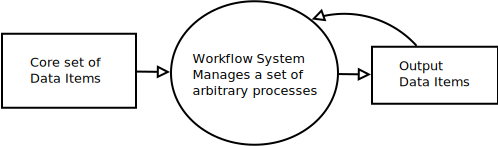
\includegraphics[scale=0.34]{figures/basic_system.pdf}
		\end{center}
		\caption{Basic System Overview}
		\label{intro:basic}
	\end{figure}

	\noindent The system would starts with with
	core set of input files. The workflow is then executed which initiates a set
	of topological tasks. These tasks would then be executed in order, such that
    the processes then generate the full set of output data items.

    These processes can be ordered into two main categories:
    \begin{inparaenum}[i)]
        \item tasks that can be automatically be executed by the system and
        \item tasks that need to be completed by a user
    \end{inparaenum}. The system aims to coordinate an automate these tasks to
    the maximum extent possible whilst managing the information at this
    scale.

    Executing these processes involves using a various software packages.
    This functionality can not be replaced by the system so it would need
    to be integrated in a very general way.

\section{System Evaluation}
    In order to determine the applicability of the proposed solution, the system
    was evaluated in the following way:

    \begin{description}
        \item[Partial Integration]\hfill \\
            In order to determine whether the proposed system
            would be applicable to the problem at hand, a portion of the workflow
            of and existing site was implemented and tested within the system. This
            test provides a mean to determine whether the problem could be solved
            by the proposed system.
        \item[User Experience Testing] \hfill \\
            Even the most effective system can fail if it cannot
            be successfully be adopted be users. Therefore the system's
            user experience was tested. This allows problems to be detected and
            shortcomings of the system to be identified\cite{tullis2008measuring}.
    \end{description}

\section{Legal and Ethical Issues}
    All the software used in the development of the workflow system
    is either free or open source. If this project were to continue
    or be extended there would not be any legal issues. The core
    of the system is written using the Django Framework, using Python
    These are respectively licenced by the Django Licence and the PSF
    license. Further tools used during the implementation include Javascript,
    JQuery, JsPlumb, and tablesorter. Which is licenced under LGPL,
    MIT license and GPL version 2.

    User testing was also done during the course of the project, from
    this purposes Ethical clearance was granted from the Faculity of
    Science Research Ethics Committee. Access to UCT Students was also
    granted by the Department of student affairs.

\section{Document Outline}
    This report outlines the design, implementation and evaluation
    of \emph{Zamani Workflow} a workflow system that sets out to
    solve the data management problem experienced within the
    Zamani Project. The report starts with a review of the literature in
    Chapter~\ref{chap1}.

    This is then followed by the Design and Implementation of the system
    in Chapter~\ref{chap2}. The considerations for the design are defined
    before the full system design is reported throughout the three design
    iterations.  The system in then evaluated in Chapter~\ref{chap3}.


\chapter{Background\label{chap1}}
    Workflow management systems define a complex process in into well formed
    tasks and coordinates the process completion \cite{1245778}.  Automated
    workflow management has been in wide use across various disciplines since
    the concept was formalised in 1996\cite{springerlink:10.1007/BF00136712}.
    Successful systems have been implemented across various fields including
    banking, pharmaceuticals and various others
    \cite{Brahe:2007:SWW:1316624.1316661,5407993}.

    It has been shown to be very successful the sciences as the same scientific
    process can easily be repeated on a different set of data\cite{4721191}.
    This not only aids in reproducibility but also saves time.  This is done by
    efficiently abstracting the operations in the flow, allowing it to be
    automatically handled.

    Geomatics is the field that concerns itself with the organisation,
    representation and processing of geographic data, for the purpose of
    querying it and making decissions off of the data
    \cite{DiMartino:2007:TAG:1341012.1341081}. The workflow in Geomatics is
    very distributed and the set of data that is operated on is large and
    diverse.  Workflow management within Geomatics has been considered and
    solutions have been proposed, but not implemented or
    evaluated\cite{Migliorini:2011:WTG:1999320.1999356}.


\section{Overview}
A workflow management system consists of definitions on how a set of tasks
should be executed \cite{springerlink:10.1007/BF00136712,vanderAalst2002125}.
The overall procedure is defined by the following components:
\begin{inparaenum}[(i)] \item actors, \item roles, \item responsibilities and
obligations, \item tasks, \item activities,\item conceptual structures and
\item resources.\end{inparaenum}

A real life problem or task can then be broken up into these components in
such a way that the tasks represent a flow network. These tasks then connect to
the actors and resources via the other
components\cite[p.~4]{Taylor:2006:WES:1196459}.  This allows task to be
executed efficiently in a distributed manor.

The initial implementations of a workflow system, however, almost
immediately failed. The system was too rigid and was unable to accommodate the
high levels of change that was required by the users
\cite{Suchman:1983:OPP:357442.357445}.

These changes come from a number of sources, including: ill-specification
of initial problems, change in actors or resources, exceptions that occurred
and new requirements.  Adaptive workflow systems were proposed to solve this
problem by providing a mechanism for allowing change in the
system\cite{vanderAalst2002125}. This allows processes to be extended, replaced
or re-ordered. It also adds the ability to change already running tasks by
providing restart, transfer and proceed options.

Scientific workflow management has also been very successful with how
experiments are defined, and more importantly, reused. Another benefit that was
quickly discovered was that it also allowed researchers to trade workflows,
making the replication of results much easier than they were
previously\cite{4721191}. Keys to this success were: that the workflow systems
were made to fit the researchers, quick responses to adding required features
when needed, listening to user input and making sharing of workflows as easy as
possible.

Such a system has also been applied in fields that operate on large data
sets, as would be the case if applied to problems in Geomatics
\cite{Aragon:2009:WMH:1529282.1529491}.  Workflow systems were found to
work well in the management of getting this data processed. Applying the
concept to Observational astrophysics, it revealed that it could be used to
identify bottlenecks that could be optimised.  Further it was used to
automatically ensure local access of large files that needed to be processed.


\section{Geographic Data}
Geomatics concerns itself with the collection, organisation and query of
geographic data \cite{DiMartino:2007:TAG:1341012.1341081}.  This data includes
but  is not limited to landscapes, coordinate data, building models,
statistics, pictures, textures and routes. This is a very broad set of data,
varying from very large to very small.  That variation however, means that
there exists no uniform method to efficiently deal with the data.

The processing of this data can vary from human to software processing
\cite{DiMartino:2007:TAG:1341012.1341081}.  Various Web applications have been
written to facilitate the tasks that need to be accomplished.  This software is
known as WebGIS and is becoming more popular with scientists; it also means
that even within the field there is a strong shift toward Web based services.

A key realisation with the usage of this data is that the same data is used
across various applications, to create various amounts of
abstractions\cite{ElAdnani:2001:MLF:512161.512177}.  The core data is seldom
changed. Instead a new abstraction layer is added on top of it. The data can be
thought of as a graph, where the nodes represent either a data or abstraction
element, and the edges represents the functions/tasks required to create the
particular abstraction as a set of topological relationships. This can be
effectively used to provide high levels of interoperability.

\section{Implementations}
There are various products available that can compose scientific workflows.
\emph{The Trident workbench} \cite{Simmhan:2009:BTS:1673063.1673121} is an open
source workflow management system developed by Microsoft Research that also
adds middleware services and a graphical composition interface. Trident builds
workflows of control and data flows, off of built-in, user defined activities
and nested subflows.

The flows are represented using XOML, an XML Specification, while the
activities are stored as a set of sub routines\cite{Simmhan2011790}. Trident
can be used on a local system, remote systems and even clusters.  Queries on
the system can be performed using LINQ.


\emph{Kepler} is another scientific workflow management system that
provides workflow design and execution.  Actors are designed to perform
independent tasks that can either be atomic or  composite
\cite{Wang:2009:KHG:1645164.1645176}.  Composite actors(subflows) consist of
multiple   atomic actors bundled together. Actors can consume data and produce
output, called tokens. Actors communicate tokens with each other via links. The
order of execution and the links are defined by an independent entity called
the director. As a consequence, the workflow can either be executed in a
sequential or parallel manner. Kepler effectively separates the workflow from
its execution, allowing for easy batch execution. Actors can easily be exported
and shared.  Kepler is very popular due to its adaptability and easy
integration.

    \emph{Taverna} is a scientific workbench that supports application-level
workflow and does not focus on scheduling as much others\cite{4721191}. Taverna
has a strong focus on workflow sharing. Taverna is quite popular, since there
exists a social network, designed to facilitate workflow sharing among
scientists(\emph{myExperiment}). Services are linked to the model to execute
the various tasks. Taverna can be used in such a way that it can utilize all
the services a client has to facilitate the flow by easily adding services. The
Taverna language is a simple data-flow language called the Simple Conceptual
Unified Language(SCUFL), that can be encoded to XML.

In order for these workbenches to be successful, there needs to exists a
high level of interoperability between the workflow management and the services
that are required \cite{Shegalov:2001:XWM:767132.767139}.  However, due to the
fact that there is a relatively high chance of failure when building this
interoperability into the services as a core component. It is an extremely high
risk and therefore is not typically done. A Cheaper way of doing this is
providing middleware that can wrap around the service to provide the required
interfaces.

This need for interoperability has led to the popularisation SOA(Service
Orientated Architecture) \cite{Sanders:2008:SSA:1400549.1400595}.  It should be
noted that SOA is \emph{not} an implementation, but rather an
\emph{Architectural Model} SOA refers to a collection of loosely coupled
services, that individually carry out a particular process. Each service should
have a well defined interface with self-contained functionality. It should
allow other applications or services to use this functionality without knowing
the underlying technical details. These services should be hidden from the
end-user and its usage should preferably be platform-independent.

Although the concept has been around since the 1970s, it has only recently
gained favour due to Web services.  Web services are software that run on the
internet through XML standards-based
interfaces\cite{Tai:2004:CCW:1045658.1045680}.  Each service provides a
fuctional description using the \emph{Web Services Description Language}(WSDL).
This description provides the supported operations, as well as the definition
of the input and output messages.

By using these concepts, a workflow system can be built that automatically uses
these Web Services to facilitate both the data and control flow using well
defined interfaces in standards such as XML/JSON.
\cite{Shegalov:2001:XWM:767132.767139}. With the advancement of WebGIS, a lot
of Web Services that facilitates Geomatics processing already exists.


\section{Case Studies}
The next section will look at two instances where workflow management systems
were implemented and used.  These case studies will look at both a business and
a scientific application.
    \subsection*{Danske Bank}
      The workflow management system at \emph{Danske bank} was incrementally
      implemented as their system moved from a manual
      system\cite{Brahe:2007:SWW:1316624.1316661}.

      This system was developed as an in-house solution when the manual system
      could not cope anymore.  Several lessons were learnt that are applicable
      to other work flow systems. When work was divided purely from an
      efficiency point of view, the workers became complacent as they felt that
      they did not understand the overall mechanism and felt that they were not
      involved. They discovered that the system did not handle change very
      well. This change was expensive and inevitable. Their system had to be
      adapted to handle this change. The success of the system is mainly
      attributed to the interoperability and close relationship between the
      users and the developers

    \subsection*{OrthoSearch}
      \emph{OrophoSearch} is a workflow, built on \emph{Kepler}, that is
      designed to work on work on data in the field of Bio Informatics.
      \cite{daCruz:2008:OSW:1363686.1363983}

      A workflow system was implemented in \emph{Kepler} as it addressed the
      requirements they had, including: \begin{inparaenum}[(i)] \item Workflow
      definition and Design; \item workflow execution control; \item fault
      tolerance; \item intermediate data management; and \item data provenance
      support.  \end{inparaenum}

      Although the system was not without its hiccups and changes, the
      integration with Kepler provided the workflow increased overall
      productivity.


\section{Implication}
The field of Geomatics concerns itself with a vast amount of geographic data.
This data comes in various sizes and as such different methods of handling and
transferring would need to be used to facilitate dataflows within the system.

The work however is done in a very distributed manner, which allows for a very
effective mapping onto a grid-based computing solution, provided middleware can
be developed to support the systems that are
used\cite{Montella:2007:UGC:1272980.1272995}. This would allow for an
effective Content Delivery Network that provides data on demand where it is
needed on the grid.

Workflow for Geomatics processes, due to its distributed nature, would map well
onto a automated workflow system

\cite{Withana:2010:VWE:1851476.1851586}. The nature of the science is supported
well. It would allow for effective automation of some of the functions are
available.

\chapter{Design\label{chap2}}
\section{Introduction}
The  system was implemented in three design iterations. These iterations are
as follows: \begin{inparaenum}[(i)] \item Feasibility design;
\item Workflow system design; and \item User Interface design.
\end{inparaenum} The methodology used was to design, implement
and evaluate the system at each iterations. The evaluation at
each step was then used as additional input at the following
design step. This is illustrated in Figure~\ref{design_figure}.

\begin{figure}[!h]
\begin{center}
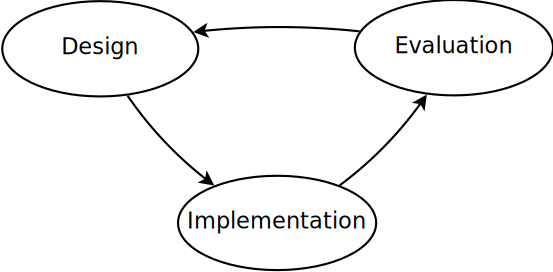
\includegraphics[scale=0.5]{figures/design_cycle.pdf}
\end{center}
\caption{Design Process}
\label{design_figure}
\end{figure}

\noindent This chapter describes the design process followed in the building
of the workflow system. Section~\ref{design_consdierations} describes
the items taken into consideration in the initial design. This was then
followed by the process used during the first iteration in Section~\ref{feasibility}.
Section~\ref{iteration2} follows with the design and implementation of the
first functional product; this product was then evaluated using user a small
group of test users.
The final design iteration was done by correcting the criticisms that test
experiences with the system. During Section~\ref{iteration3} the final
improvements and features were added in order to solve the question posed.

\section{Design Considerations\label{design_consdierations}}
This system is developed for the Zamani Project. This requires
a thorough understanding of the requirements that exist within
the team. This then has to be combined with the general requirements
of a workflow system.
\begin{description}
    \item[Workstation configuration] \hfill \\
        Within the Zamani team each member has a workstation on campus.
        These workstations vary in specification but are all locally
        connected to a high speed local network. These workstations are
        predominantly \emph{Microsoft Windows 7} based machines.  On this
        network there is also a server present. This server is used as
        a repository for the sites. Figure~\ref{network_setup} shows the setup
        of the workstations. Files required to process any particular task are
        typically transferred over the network or via removable drives.
\begin{figure}[!h]
    \begin{center}
        \includegraphics[scale=0.6]{figures/networklayout.pdf}
    \end{center}
    \caption{Zamani Network Configuration}
    \label{network_setup}
\end{figure}
    \item[Task Variety] \hfill \\
        The team's main tasks involve creating derivative data off of laser
        scans, photo graphs and other source data. A large portion of these
        tasks can be automated, whilst others require manual processing by the
        team. As such, the tasks can be divided into two types: user tasks and
        server tasks.


    \item[Dataflow model] \hfill \\
        The process involves the data constantly moving between the server
        and workstations with data elements being added at every step. These
        flows are rather complex and relate closely to the workflow of the
        project.  Given the scale of the data being processed, transferring the data
        from one end to another has a large cost. As such this cost should
        be factored into the design.


    \item[Staff Turnover] \hfill \\
        The project consists of a core number of individuals as well as
        a group of interns who cycle in and out of the project on a regular
        basis. This would have an impact at the task
        level if a user fails to complete a particular task before leaving
        the project. Due to the high staff turnover rate this would
        be a frequent occurrence and as such would have to be sufficiently
        dealt with by the system.

    \item[Repeatability] \hfill \\
        In creating this data the same processes are essentially followed
        on all sites. In the design of the processes these would need to
        be reusable on different sites with very little effort. This
        will aid in the easy repeatability of experiments.

    \item[Integration with existing software] \hfill \\
        The Zamani project uses a wide variety of programs during
        the processing of this data. The workflow system would have
	to integrate with this software as well.

    \item[System Backup] \hfill \\
        Each site consists of a set of data items. This data is very valuable
        and is often irreplaceable. In the case of a system failure
        the loss of the data would have great costs. As this system would
        be controlling these items it would have to allow for the site
        to be backed up.

    \item[Provenance] \hfill \\
        Provenance refers to the documented history of an object\cite{moreau2008open}. For
        digital objects this refers to all the objects, processes and agents
        involved in the life cycle of the object. Provenance is perceived as
        a crucial component in workflow systems. This is designed to aid in
        analysis of systems and help ensure reproducibility. The Open
        Provenance Model was designed to represent the capabilities of a system.
        This allows the technology to be defined in an agnostic way and
        allows systems such as this to be built using this model.

        This model consists of three primary entities: \begin{inparaenum}[(i)]
        \item Artifacts; \item Process; and \item Agents.\end{inparaenum} These
        artifacts are joined using relations and dependencies.
        Figure~\ref{provenance}  shows the relations between the entities of
        the model. The benefit of using such a model is that it has been
        extensively tested in other similar systems with great success.
        \begin{figure}[!hb]
            \begin{center}
                \includegraphics[scale=0.5]{figures/provenance_edges.png}
            \end{center}
            \caption{Edges in the provenance model}
            \label{provenance}
        \end{figure}
\end{description}

\section{Feasibility Demonstration\label{feasibility}}

The core focus of the this iteration to ensure that the core types of tasks
in the system would be supported. The main tasks were, user-tasks and tasks
that can be automated. During this portion a significant amount of time and
effort was spent on comparing different systems with one an other.

This phase produced a small system, that supported very primitive manual and automatic
tasks. The system was integrated with \emph{Kepler}~\footnote{
The Kepler Project: www.kepler-project.org }, and could copy over files to a remote
host. The tasks could be signaled as being: ``Not Done''; ``In Progress''; or ``Complete''.


\subsection{Design}
The initial design focussed on enabling the type of tasks required by the system.
These tasks can be abstracted into two main types: \begin{inparaenum}[(i)] \item
Manual User Tasks; and \item Automated tasks\end{inparaenum}.


The workflow-management system intends run on the same server that hosts the central
site repository. This would allow inherent data locality therefore would allow for
efficient server operations on the data. These operations would be performed on data
of a given site. Sites can be abstracted to a large hierarchical collection of data
items. To aid in the repeatability of experiments the hierarchy of each of these
sites should kept consistent both within the main repository and on the user hosts.

\subsubsection*{Server Task}
The first type of task that would need to be facilitated by the system are those
tasks that can be done automatically by the system and require no interaction
from a user. These include removing duplicate points in input data, or changing
a file to a particular format. To avoid the high cost of transferring data these
tasks are performed on the server itself.

\subsubsection*{User Task}
The second type of task that needs to facilitated within the system is manual
tasks performed by the members of the team. During such a task, particular data
elements of the site are required to create new derived data elements. As all the
team members cannot work on the server, the required files would need to be moved
to the respective workstations. Figure~\ref{data_flow} shows the data flow for any given
User task.
\begin{figure}[!h]
    \begin{center}
        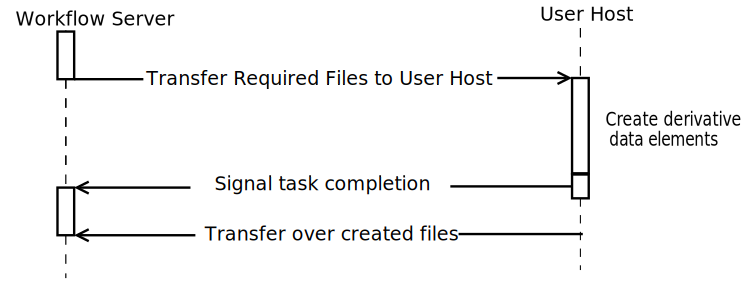
\includegraphics[scale=0.5]{figures/data_flow.pdf}
    \end{center}
    \caption{Data flow in user task}
    \label{data_flow}
\end{figure}

\subsubsection*{Basic Task Model}
These task types can be abstracted for the workflow system into a general
task type. This allows the system to handle them indiscriminately. The basic
requirements of a task are to take a set on input data and produce a set
of output data; these are mapped to artifacts in the provenance model.
This will allow the tasks to be chained together to form
a complex workflow. This task maps to the \emph{Process} entity in the
provenance model. Each task would be assigned to a assigned to a user, which
maps to an agent in the provenance model.

\subsubsection*{Kepler integration}
Kepler is a popular workflow system, with pre-built models to
facilitate complicated workflows. Ideally the system would need to be able
to integrate with Kepler so that it can harness the existing capability
of the system.

\subsubsection*{Site Layout}
Within the Zamani Project the data is organised at the root level in terms of
the physical site with which the data corresponds. Since the goal is to have the
tasks executed on a variety of different workstations, the data management
would be greatly simplified if the folder structure is the same on the workstations
and the server. For this reason workstations and the server will have
an identical directory structure with the site being regarded as the root. This
layout could be changed from site to site to allow for more flexibility.

\subsection{Implementation}

The first round of implementation set out to test the feasibility of the
core components required within the system. As shown above, this is identified
as setting up the framework for the User and Server Tasks. This was done using
Kepler, Java, and a series of command line tools. This was split into the following
components: \begin{inparaenum}[(i)] \item Database; \item Kepler Task Model;
\item and a Kepler File Copier. \end{inparaenum} These could then be packaged
to create complicated workflows that could represent a site.
Figure~\ref{iter1_overview} shows how these components interact with one another to form the core components of the workflow system.

\begin{figure}[!h]
    \begin{center}
        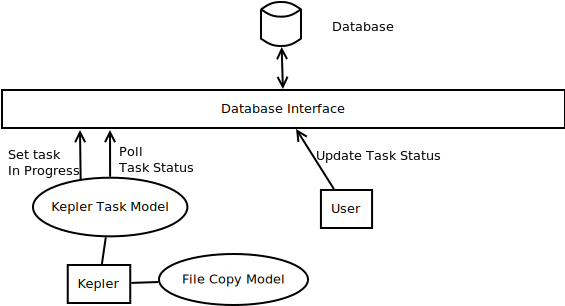
\includegraphics[scale=0.35]{figures/iter1_impl.pdf}
    \end{center}
    \caption{Feasibility components}
    \label{iter1_overview}
\end{figure}

\subsubsection{Database}
In order to keep track of the tasks, a MySQL database was used. Tasks could be added
to the database along with a status. As a task progressed thorough the process its
status would be updated, which would trigger events in the system. Initially tasks would
have three valid statuses: ``NOT DONE'', ``IN PROGRESS'' and ``DONE''. The database would
be updated by small scripts that could be called by Kepler.

\subsubsection{Kepler Task Model}

This model is used to launch user tasks. The model then polls the database for
status changes of the task. As soon as a user completes the task the
database is updated, the model would pick this up and continue with the process.
Figure~\ref{kepler_task_model} shows the workflow in Kepler for the task model.

\begin{figure}[!h]
    \begin{center}
        \includegraphics[scale=0.6]{figures/task_model_kepler.png}
    \end{center}
    \caption{Kepler model that launches a user task}
    \label{kepler_task_model}
\end{figure}

Kepler is not ideally suited for user-tasks as its primary focus is complex
automation. It is also highly suboptimal as it needs to
continuously poll to determine the status of a given task.

\subsubsection{Kepler File Copier}
User tasks also need files to be copied to the user workstations. For this
a Kepler workflow was built that copies files. Each task has a list with the
files required to complete the task. The model uses SCP to copy over files
to the respective user. Figure~\ref{kepler_file_model} shows how the model
is built in Kepler.

\begin{figure}[!h]
    \begin{center}
        \includegraphics[scale=0.6]{figures/kepler_file.png}
    \end{center}
    \caption{Kepler model that copies files to workstations}
    \label{kepler_file_model}
\end{figure}


\subsection{Evaluation}
Due to the lack of functionality of the first prototype the first
phase of evaluation was rather short. This prototype was demonstrated to
the second reader (Dr. Bagula). The prototype showed that the core
requirements could be implemented and was critical to develop a more
complete understanding of the problem.


\subsubsection{Dropping Kepler}
Kepler is rather bulky and the user task model is ill-suited to the system.
The Zamani Project's tasks fit better to an operational model, whereas Kepler
is suited to more scientific data processing model.

Kepler also does not integrate very well from an interface point of view.
As such it was decided that Kepler would not be used in the next iteration. This
requires that its functionality be replicated in the next iteration.

\section{Functional Design\label{iteration2}}
This section follows the second design iteration using the first iteration
as a base. The goal of this iteration is to create a workflow system that is
functionally adequate to support the automation of the workflow for the Zamani
Project.

\subsection{Design}
The design of the second iteration follows a more rigorous process and has the
primary goal of supporting most of the required functionality. The system should
be support multiple users, each being able to execute a portion of the workflow
assigned to them.
\subsubsection{Web Interface}
Using a web interface is well suited to the problem. This will allow multiple
users to log in, track and manage their tasks. This could also be hosted on the
same server that would host the primary site repository. Preference and prior
experience experience led to the adoption of Django\footnote{Django Web Framework
www.djangoproject.com} for this purpose. Django is a Python framework that allows
for rapid Web application development. Due to the type iteration cycles Django is
well suited to be used as the supporting framework for the system.
\subsubsection{Replication of Kepler functionality}
The feasibilty demonstation showed that Kepler has poor support for the user
tasks required within the workflow system. This functionality will need to
be replicated within the new framework. This requires classification
of the Zamani workflow such that it can be correctly implemented.
A workflow management system can be classified by four different elements
\cite{yu2005taxonomy}:
\begin{description}
    \item[Workflow Design] \hfill \\
        The tasks required within the project are well defined.
        Data is transformed in a linear manner. Data items do not get iterated over
        once they are complete. Therefore the system would fit a user defined,
        directed acyclic graph. This workflow would be designed by the user to
        allow for arbitrary dependencies.
    \item[Workflow Scheduling] \hfill \\
        Based on the way that the project is currently executing tasks, the scheduling
        would need to happen dynamically with a priority to determine the
        urgency of any particular task.
    \item[Fault Tolerance] \hfill \\
        Since the system would be dealing with a large amount of data, a lot of which
        will be generated by the users themselves, the likelihood that tasks may fail
        is quite high. Therefore it needs to be mediated. Since the workflow models
        would be manually created by a user, workflow level errors will not be taken
        into account. The system will however have to be able to deal with task level
        failures. The mediation process would include: the ability to retry a task
        and modify the node on failure. Both of these would have to be mediated manually
        by the user.
    \item[Data Movement] \hfill \\
        New data items is continuously generated and as such the movement of the data needs
        to be controlled. The goal is to automate the data movement, using a centralised
        repository that maintains the authority on data.
\end{description}
Django is built using Python and uses a \emph{Model View Controller}
architecture\cite{leff2001web}. This model separates the system into three parts: the
data, the control logic and the presentation of the data. The MVC framework would allow for
the workflow logic to be built and executed independently of the User representation of it.

\subsubsection{Participatory Design Session}

To ensure that the product meets the needs of the client they were made active participants
in the design process. The methodology used during this is Participatory design
\cite{muller1993participatory}. Due to limited time this was selectively applied.
Four members of the Zamani Project were
brought together for a PICTIVE design session \cite{muller1991pictive}.
The method used can be outlined as follows:
\begin{inparaenum}[(i)]
\item General Requirements gathering;
\item defining the task flows; and
\item a graphical user interface PICTIVE design session.
\end{inparaenum}

The session identified the core tasks that need to be supported. These
include the following:
\begin{itemize}
    \item Workflow Setup
    \item Template Functionality
    \item Progress Indicators
    \item Task time information
    \item Task control from a user perspective
    \item Logging Functionality
\end{itemize}
These tasks were then further developed to create a logical use-case. The
most important functionality defined were as follows:
\begin{description}
    \item[Task Definition] \hfill \\
        The focus was on what users would need regarding tasks.
        The suggestion was made that all tasks be separated at site level.
        Each task should have the following properties:\begin{inparaenum}[(i)]
        \item Name; \item Priority; \item Category; \item input files; \item
        status; \item description; and \item an output directory
	\end{inparaenum}.
        Users should see an overview of their tasks, and on demand be able to
	obtain
        further details on a particular task. Tasks would be assigned to users.
        User Tasks performed by unprivileged users should also be checked by
        privileged users before being checked as complete. Users should be
        able to re initiate downloads of the required files to their hosts.

    \item[Task Setup] \hfill \\
        In order to set up the workflow, an administrative interface is required.
        This should allow for the creation of tasks. Each task would have a set
        of dependencies, linking to other tasks that need to be completed before
        the task can start. It would also require a graphical overview of the
        site's task. From this view users should be able to add and edit tasks,
        having access to all the parameters of the task. Each task would have
        a separate log allowing users to determine what the causes of failures are.
	Sites should be able to have an initial set of tasks populated using a
	previous site as a base. This would allow workflows to be reusable, which
        is preferable as each site follows roughly the same process. The
	workflow for the derived site can then be modified independently to
	allow for site specific conditions.
\end{description}
The final task of the session was to create a mock user interfaces for the
identified tasks. This was using low-fidelity items, which included small pieces
of paper that represented the components that need to be added. This activity
was performed with a small group of users who are involved with the Zamani Project.
Three screens were set up.

Figure~\ref{pictive_site} contains the controls for each site. The main component
on this screen is the visualisation of the workflow. Below this is a table that
contains a list of all the tasks in the site. Controls to add tasks and categories
were also added. The tasks to edit and add tasks should only be available to privileged
users. The second screen developed is aimed to give an overview of the
the tasks. Figure~\ref{pictive_tasks} is separated into two sections. The top
section contains a list of the tasks that are outstanding. The bottom  portion
contains a list of tasks that are currently in progress by the rest of the team.
An additional feature is a progress bar that indicates the progress of the
completed tasks. The last screen that was developed during the session was the task control
screen. Figure~\ref{pictive_task} gives a detailed description of task. It should
allow users to indicate their task's completion. With the correct permissions,
users should be able to validate completed tasks of general users within the
system.

\begin{figure}[!h]
\begin{minipage}[b]{0.48\textwidth}
    \begin{center}
        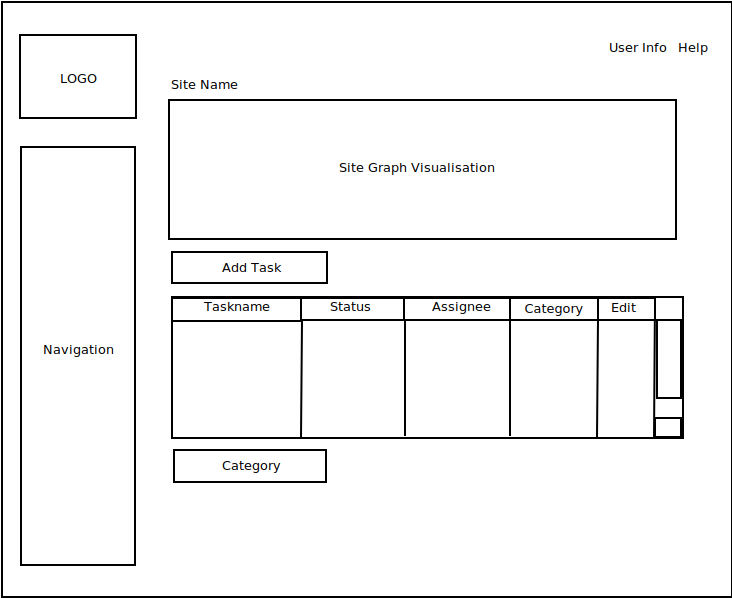
\includegraphics[scale=0.25]{figures/site.pdf}
    \end{center}
    \caption{Site screen developed during the PICTIVE session}
    \label{pictive_site}
\end{minipage}
\hspace{0.5cm}
\begin{minipage}[b]{0.48\textwidth}
    \begin{center}
        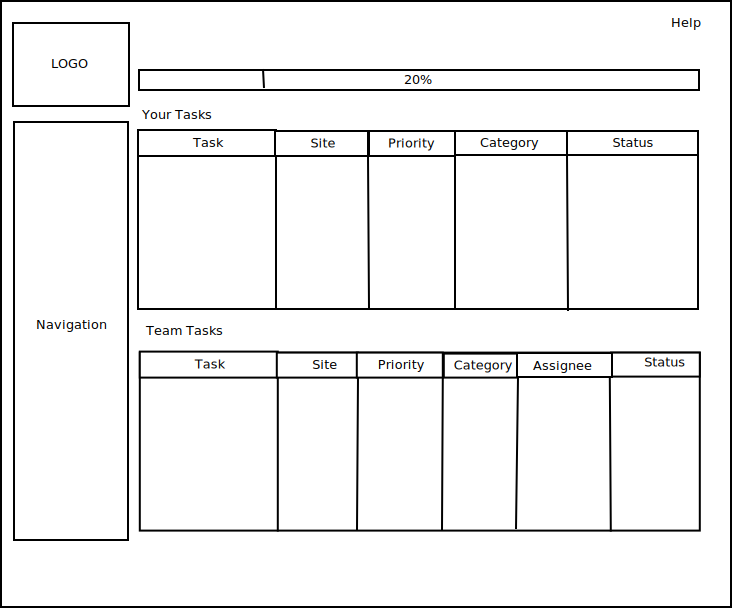
\includegraphics[scale=0.23]{figures/task_list.pdf}
    \end{center}
    \caption{Task Overview screen developed during the PICTIVE session}
    \label{pictive_tasks}
\end{minipage}
\end{figure}

\begin{figure}[!h]
    \begin{center}
        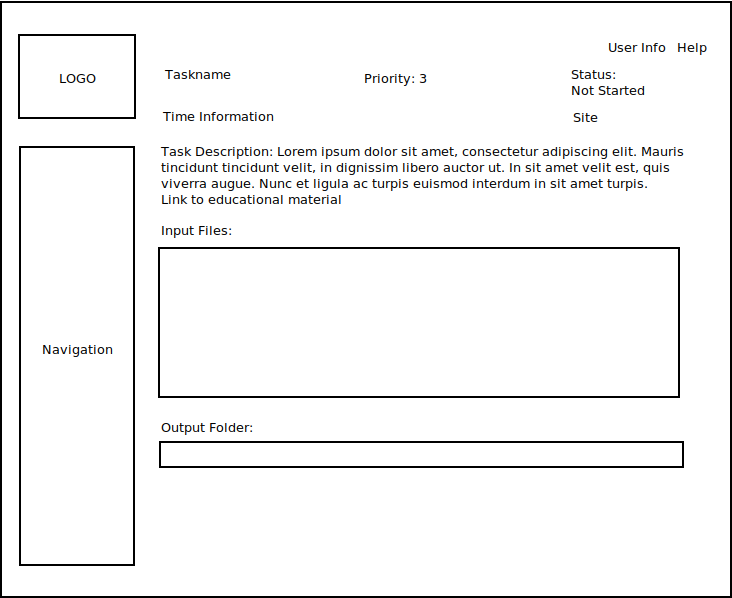
\includegraphics[scale=0.25]{figures/task_overview.pdf}
    \end{center}
    \caption{Task Control screen developed during the PICTIVE session}
    \label{pictive_task}
\end{figure}

\subsubsection{Database Schema\label{db_schema}}
The system needs to manage a large amount of data. This requires
a database that will control all the information required for the
workflow system to function. The primary tables required for this are:
\begin{inparaenum}[(i)]
\item Sites;
\item Jobs;
\item Hosts;
\item Files; and
\item Tasks.
\end{inparaenum}

\noindent Each of these tables is described below:
\newpage

\begin{wrapfigure}{l}{7cm}
\begin{tabular}{l|l}
    \multicolumn{2}{c}{Site} \\
    \hline
    Name        & Type \\
    \hline
    Id          & VARCHAR(30) PK \\
    Name        & STRING \\
    Folder Name & STRING \\
    Active      & BOOLEAN \\
\end{tabular}
\caption{Site Schema}
\end{wrapfigure}
\noindent\textbf{Site:}
This table stores the root information for the various sites that
the project is working on. The ``Id'' field is used for short
\emph{URLs}, while ``Name'' is used for display puposes. ``Folder Name''
provides the root folder that the site data will be stored in. This
allows for consistency between the repository and the client workstations.
As soon as a site is completed it will also have the option of being marked
inactive. This will prevent the clutter of old sites that no longer require
workflow to be managed.
\\
\begin{wrapfigure}{l}{7cm}
\begin{tabular}{l|l}
    \multicolumn{2}{c}{Job} \\
    \hline
    Name        & Type \\
    \hline
    Id          & AUTOINT PK \\
    Name        & STRING \\
    Type        & CHOICE \\
    Script      & PATH \\
    Description & TEXTFIELD \\
\end{tabular}
\caption{Job Schema}
\end{wrapfigure}

\noindent\textbf{Job:} This table was created to help tasks to be more reusable.
The purpose of a given task will be determined by the \emph{Job} that the task
is linked to. This table supports three main type of jobs, namely:
\begin{inparaenum}[(i)] \item User Jobs; \item Server Job: one-to-one; and \item
Server Job many-to-one.\end{inparaenum} This is represented by the type field.
For server tasks the \emph{Script} field is set to a path that contains the
server side script that will execute on the input files defined within a \emph{task}.
For one-to-one tasks  the script is executed once per input file, while it
is executed only once for many-to-one jobs. Information about the job is stored
in the \emph{description} field. The rest of the fields are used to facilitate
naming and queries.
\\
\begin{wrapfigure}{l}{8cm}
\begin{tabular}{l|l}
    \multicolumn{2}{c}{Host} \\
    \hline
    Name        & Type \\
    \hline
    User        & FOREIGNKEY(User)  \\
    Host Name   & STRING  \\
    Root Directory & PATH \\
    Primary      & BOOLEAN \\
\end{tabular}
\caption{Host Schema}
\end{wrapfigure}

\noindent\textbf{Host:} This table manages the control of a user's workstation.
The \emph{user} field points to the user attached to the particular host. The
\emph{hostname} contains the connection string that connects to the user's workstation.
Since every user is likely to have a different folder structure on their workstations,
a \emph{root directory} field was added to indicate a path on the workstation that
will be used as the root folder for the sites. It is very likely that a user could
have more than one workstation, therefore a \emph{primary} field was added to indicate
which host would be the default for that user.
\\

\begin{wrapfigure}{l}{7cm}
\begin{tabular}{l|l}
    \multicolumn{2}{c}{File} \\
    \hline
    Name        & Type \\
    \hline
    Filename    & PATH  \\
    Site        & FOREIGNKEY(SITE)  \\
\end{tabular}
\caption{File Schema}
\end{wrapfigure}
\noindent\textbf{File:} Each file will have a database entry.
This will add the ability of a quick file lookup and aid in maintaining files between the
repository and the workstations. Each entry will have a \emph{filename}: this will store
a relative path from the site root to the file name. By only storing the relative path
we are able to access the file without making assumptions on where the root directory
is. The second field links a file to the site that it belongs to.
\\

\noindent \textbf{Task:} This controls how the workflow is put together in the system.
Each task is defined as an independent activity that can be executed by the server or
by a user. Each task has a list of dependencies that need to be satisfied in order
for the task to be executed. When a task is complete its successors are then checked,
and run if all the dependencies are met. In order to ensure that this can be
done efficiently,
both the predecessors and the successors are stored in the table. The \emph{Id} field is
used for task identification in URLs. Each task also has time information, the execution
time of a

\begin{wrapfigure}{l}{7cm}
\begin{tabular}{l|l}
    \multicolumn{2}{c}{Task} \\
    \hline
    Name        & Type \\
    \hline
    Id              & AUTOINT PK  \\
    Priority        & INTEGER  \\
    Started         & DATETIME \\
    Ended           & DATETIME \\
    Log             & TEXTFIELD \\
    Site            & FK(Site) \\
    Job             & FK(Job) \\
    Assignee        & FK(User) \\
    Input Files     & MTM(File) \\
    OuputFolder     & PATH \\
    Predecessors    & MTM(Task) \\
    Successors      & MTM(Task) \\
    Job Status      & CHOICE FIELD \\
\end{tabular}
\caption{Task Schema}
\end{wrapfigure}
\noindent task can be calculated by subtracting the start time from the end time. Each
task is based on a \emph{Job}: this allows jobs to be reused in various tasks, making the
system easier to use. A task is explicitly assigned to a user; for automatics tasks a
dummy user named ``server'' is used to ensure database consistency. The input-files of
a task is defined in a ``Many-to-Many''\footnote{MTM refers to Many-To-Many Field}
field; this enables the system to only transfer
required files to workstations as well as running the script on appropriate data. When
a task is executing, the system expects the output files to be placed in the output folder
field, this allows the system to manage the file dependencies of the successor tasks.

Along with the system being failure tolerant, it also needs to be able to determine what
has happened when a failure has occurred. For this reason a \emph{Log} field was
added. This field stored all the activity that a task performs. This includes the transfer logs as
well as any output generated during the execution of the server scripts. Tasks are also
stateful; this state is represented by the \emph{Job Status} field. The possible states
for a task are:
\begin{inparaenum}[(i)]
\item NOT DONE;
\item TRANSFERRING;
\item IN PROGRESS;
\item TRANSFERRING BACK;
\item VALIDATION REQUIRED;
\item DONE; and
\item FAILED.
\end{inparaenum}

\subsubsection{Features}
All these components were put together to support the required features of the system. Below
are a list of features that were implement during this design iteration.
\begin{description}
    \item[File Transfer] \hfill \\
        User tasks are able to transfer files to the user workstations, from the input
        file list. As soon as a user task is triggered the file list is retrieved
        from the task entry. The server then connects to to the host and copies over all
        the required files. Since a user can have more than one host, this transfer can also
        be manually triggered by the user. When a task is then completed the server will
        again initialise the file transfer but in the opposite direction. This
	will upload all files that are present in the \emph{Output Directory}. In order
	to support switching of workstations,
        this process can also be triggered at any stage, before the task is completed.
        Extra functionality is also added to download all the files in the output directory
        located on the server.
    \item[Task Automation] \hfill \\
        The system's ability to facilitate workflows is entirely dependent on its ability
        to automate tasks. This is done by adding a control system within the server
        that works out which tasks have no unmet dependencies. As soon as these tasks
        have been determined an asynchronous task is launched to run the task. Depending on
        the type of job, either files are transfered or a script is run. When a task is
        completed, either by verification or the script finishing, the task is finalised.
        This process involves adding all the generated files to the database, updating the
        input files of the successors. If all the dependencies of a successor
	are met that task is then started. When a task fails, however, a user is able to
	make the required changes and restart the process.
    \item[Logging] \hfill \\
        Logging is added to help with identifying and controlling task failures. Within
        the automation framework all events happening with the task are added to an
        append only log field. This includes the transfer logs for user tasks, and both
        \emph{stdout} and \emph{stderr}.
    \item[Site Visualisation] \hfill \\
        The tasks for a site can be represented as a \emph{Directed-Acyclic-Graph}. To
        make the system  more usable, the tasks will be represented as
        graph within the interface. This is done by calculating the graph of
        the sites and then applying a layout algorithm to it. For the purposes of this
        visualisation, a spring layout is used. The nodes are then joined by edges. A
        summary of each task is displayed on the node.
    \item[Site Setup] \hfill \\
        Privileged users should be able to compose workflows with relative ease. Options
        are added to allow users to create new \emph{Jobs} and \emph{Tasks}.
	Once a task is added, dependencies can then be added in a visual way on the
	visualisation. Workflows between sites are very similar;
        creating a new workflow for each site would be very time consuming. An additional
        feature is added that copies over the structure of an existing site.
	Once the new site has been built, a user would just be required to
	select the input files an assign tasks to users.
\end{description}

\subsection{Implementation\label{iter2_impl}}

The system was implemented using the \emph{Django framework}. This was done in three parts:
\begin{inparaenum}[(i)]
\item database setup;
\item workflow framework; and
\item user interface.
\end{inparaenum}

The \emph{database} was set up using the model subsystem in \emph{Django}, from the chosen schema.
This is a system that defines the database using Python; this allows the schema
to be implemented without needing to worry about the database system being used. For the
purpose of this iteration, \emph{SQLite}\footnote{SQLite: www.sqlite.org} was used to
support the database. This can however easily be changed to a more robust system as the demand
on the system grows. User data was implemented using the authentication module in Django. This
module manages users and permissions on the system. As the schema was discussed in Section~\ref{db_schema}
it will not be discussed further.

\subsubsection{Workflow Framework}
The underlying workflow system is implemented using \emph{Python}\footnote{Python: www.python.org}, within
the Django framework. Tasks are executed asynchronously. Each job type is handled separately.
\begin{description}
\item[Server Job - One to One] \hfill \\
    This job type executed a given script on all the input files. The system generates a list of
    absolute paths and executes the script given two parameters: the input file, and the output
    directory. This is done for all the input files of the task.
\item[Server Job - Many to One] \hfill \\
    This job type executes nearly identically to the \emph{One to One} task;
    however, instead
    of the script being run run multiple times, it is run once. Here however all input files
    are passed in as arguments, along with the output directory. Both server jobs can use
    any script or applications available on the system. With applications where the parameter
    structure does not match the required utility, wrapper scripts can be used.
\item[User Job] \hfill \\
    This type of job is split into multiple parts. Since there is a distinct separation between
    the server and the execution type task, the goal is to ensure the effective communication
    between workstations and servers. The goal is to be able to transfer large amounts of files
    with minimal redundancy. For this reason \emph{rsync}\footnote{Rsync Incremental file
    transfer: rsync.samba.org} is used. This only transfers files that have not been been transfered
    yet. Redundancy is greatly reduced, and this enables efficient recovery in case of network failure.

    Figure~\ref{user_task_impl2} shows the components used to execute a user task. Each of these components
    are built using an asynchronous object. Note that the transfer components can be used at any point
    during the task's life cycle.
\end{description}
\begin{figure}[!h]
    \begin{center}
        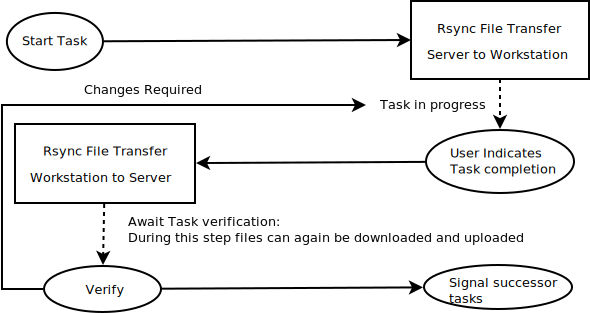
\includegraphics[scale=0.35]{figures/user_impl2.pdf}
    \end{center}
    \caption{Components that support user jobs}
    \label{user_task_impl2}
\end{figure}
    Once a task is finished it passes on to finalisation. All tasks follow this model. It
    is assumed that all the appropriate files are present on the server at this point and
    that the task has completed successfully. At this the output directory is scanned for
    files recursively, new files are indexed and added to the database. The new files are then
    added to the input files of all successor tasks. If all the dependencies of a successor
    task is met the task  are then launched.

\subsubsection{User Interface}
The interface was implemented using \emph{HTML} served using the View subsystem in Django.
These views aim to create a usable system. These are based on the designs that were created
during the \emph{PICTIVE} session. Slight alterations were made to the design to support
necessary functionality that was not considered during the session. The interface comprises of several
views.
\begin{description}
\item[Task Overview] \hfill \\
    \begin{figure}[!h]
        \begin{center}
            \includegraphics[scale=0.4]{figures/task_overview_impl2.png}
        \end{center}
        \caption{First implementation of the task overview screen}
        \label{task_overview_impl2}
    \end{figure}
    This view has shows a user which tasks are outstanding, as well as show what is
    happening within the team. This also provides links to the task control page for each task.
    An additional feature that was implemented allows users to filter tasks based on a choice
    of sites.
\item[Task Control] \hfill \\
    \begin{figure}[!h]
        \begin{center}
            \includegraphics[scale=0.35]{figures/task_control_impl2.png}
        \end{center}
        \caption{Task Control Implementation}
        \label{task_control_impl2}
    \end{figure}
    This is the view that non-privileged users will be interacting with most often. It provides
    a detailed overview of what is required to be done with the task. Privileged users also
    get a link to edit the task. This page also contains tools to allow users to download
    and upload required files. Once a user is finished with the task at hand he/she can
    simply click on the \emph{Finish Task} button. This triggers the transfer back routine
    and queues the task for verification. Users who are able to verify the task will use the
    same view, however the \emph{Finish Task} button is replaced with two buttons that will
    accept or reject the task. Logging information is also made visible to ensure that the
    complete task history is visible.

    This view is also used for server tasks. In this case the emphasis is on failure control.
    With the log visible, users can trace the source of the failure and rerun the task as soon
    as it is has been dealt with.

\item[Task Editing] \hfill \\
    During the initial task setup the parameters of a task need to be set. This screen enables
    the user to set who the task is assigned to, what the input files are, and what the task
    depends on. Note that the dependencies can also be set the task interface.
    When something goes wrong with a tasks, privileged users are also able to edit these setting
    when the workflow is already active. The workflow should be able to dynamically adapt in this case.
    \begin{figure}[!h]
        \begin{center}
            \includegraphics[scale=0.35]{figures/task_edit_impl2.png}
        \end{center}
        \caption{Task Edit Implementation}
        \label{task_edit_impl2}
    \end{figure}
\item[Site View] \hfill \\
    This view is dominated by the visualisation of the site. The visualisation
    was implemented using \emph{jsPlumb}\footnote{jsPlumb Graph UI:
    jsPlumb.org}. This is a library that builds interactive graphs. Each node
    provides an overview of the task. Dependencies are represented with edges
    while the colour of the node indicates the status of task.
    \begin{figure}[!h]
        \begin{center}
            \includegraphics[scale=0.35]{figures/site_view_impl2.png}
        \end{center}
        \caption{Site View Implementation}
        \label{site_view_impl2}
    \end{figure}
    Red indicates that there is a problem with the task, grey indicates that the task has not
    been run, blue indicates the task is in progress and green indicates that
    the task has been successfully completed. Dependencies for each task can be
    added by clicking and dragging the arrow in the corner of the node to a
    successor node.

    Below the visualisation is a list of the tasks for the site. This gives an overview
    similar to the task overview screen. A privileged user can select tasks off
    this list, which will then forward to the task editing screen.
    As soon as the tasks in a site have been set up, the workflow can be started from this view.

    The final set of components is there to add/edit jobs and categories in the system. These
    are not specifically linked to a site and can be used throughout the  system, allowing
    for easy reuse.

\end{description}
In addition to \emph{jsPlumb}, \emph{jQuery} and \emph{jQuery UI} is used extensively to build
the client side interface.
\subsection{Evaluation}
To evaluate the second iteration the system was given to five Computer Science honours students.
They were asked to critically evaluate the system. The purposes was to highlight any major
issues.

This brought up a number of issues during this iteration. The issues found are
as follows:
\begin{description}
    \item[Aesthetic Appeal]\hfill \\
    	The apparent usability is impaired by the lack of aesthetic appeal, which distracts
        from the  task at hand\cite{Tractinsky:1997:AAU:258549.258626}.
    \item[Lack of logical Flow]\hfill \\
        Some controls seem to be out of place, making their purpose hard to
	figure out; this would require some reordering.
    \item[Site Filter is confusing] \hfill \\
        The site filter appears like a button and as such its purpose is misleading.
    \item[Technical Namings] \hfill \\
        The use of technical language makes the system unsuited to a user without
        a Computer Science background. Naming should be changed to be able to include
        a wider audience.
    \item[Cycles aren't being checked] \hfill \\
        The system uses a \emph{Directed Acyclic Graph} to represent the
	workflow however; when the workflow is updated cycle checking is not done.
	This could lead a workflow to enter an   unsatisfiable state.
    \item[Allow User Specified ordering] \hfill\\
        It was noted that users cannot order tasks. This could make specific
	task very difficult to find when the list becomes increasingly large.
    \item[File Picker is too simple] \hfill \\
        The file picker is severely lacking and would be aided by using a more standard
        tree view.
\end{description}



\section{Final Design Iteration\label{iteration3}}
This iteration builds on Section~\ref{iteration2}, address the issues raised during the evaluation
phase. This iterations aims to improve usability issues encountered in the previous iteration. The
system is then evaluated for user experience by performing a user experience study with several users.
\subsection{Design}
In order to improve the usability of the system the design of the system was altered to include a
number of changes. In order to improve the overall aesthetics of the system a templated style sheet
was used. To improve the layout of the system some components were  reordered, and
changed to fit a more standard interface.

The task overview interface was reworked and the site filter was removed as it caused too
much confusion. Sorting controls was added to the task-list, allowing tasks to be located
easier. The user facing terminology was changed such that the terms a more general
and understandable to users without background in technology.

The last focus of the design was to avoid unintentional user errors.
When a user is setting up task dependencies cycle checking is be done to ensure that cycles
are not created. To further improve the usability of the system the \emph{File
Picker} was changed to a more intuitive component.

\subsection{Implementation}

During this phase several features were improved upon from the previous iteration.
These changes were all made on client side of the application and the focus was
to increase the usability and make the system more understandable.

The most noticeable change of the system is that the style-sheet was changed. The theme that
was chosen is called is \emph{Blue Nile Admin} and was designed by \emph{Portnine}
\footnote{Portnine: http://www.portnine.com/bootstrap-themes}. This is a two panel design
that roughly matches the original design. This theme also includes a range of icons which
overall makes the system more appealing.

\begin{figure}[!h]
    \begin{center}
        \includegraphics[scale=0.22]{figures/final-overview.png}
    \end{center}
    \caption{Final Implementation: Task Overview}
    \label{final:overview}
\end{figure}

The task overview screen was altered to make tasks more clear. Figure~\ref{final:overview}
shows the implementation of this. Instead of using a two table design this  esxpanded to
using separate tables tasks that have different statuses. Since \emph{outstanding tasks}
are the main points of action for users these tasks are placed in a large table on top.
Task that are \emph{awaiting validation} are placed in a smaller table below, privileged
users will also have tasks from other users appear here in order to easily see which tasks
needs validation. Tables for \emph{tasks with unmet dependencies}; and
\emph{completed tasks}, are also included. The team overview task has been filtered
to only include tasks that are currently in progress. All tables are are sortable
using \emph{JQuery: TableSorter}\footnote{Tablesorter: tablesorter.com}. Tasks can
also be filtered by site.

The file interface was changed to be more appealing and usable. \emph{JQuery Widgets}
\footnote{JQWidgets http://www.jqwidgets.com/} was used for this purpose, specifically
the \emph{JqxTree} widget. This allows users to easily select and view files in a hierarchical
manner. Figure~\ref{final:tree_view} shows how files can be views and how files can also be
selected. The selection and view interfaces are similar to be consistent throughout the system.

\begin{figure}[!h]
    \begin{center}
        \includegraphics[scale=0.45]{figures/final-interface.png}
    \end{center}
    \caption{Final Implementation: File interface}
    \label{final:tree_view}
\end{figure}

The task visualisation was changed to be visible on both the site interface, as well as the
edit interface. This allows for the removal of the unintuitive predecessor selector that
was present in Section~\ref{iter2_impl}. In the task edit interface a
specific task is selected. To indicate this the selected task will be
coloured in such a way that its stands out. The visualisation was also
changed such that task positions are static and persistent. This allows
for the tasks to be arranged by users. Figure~\ref{final:visual} shows
how the visualisation interface was changed.


\begin{figure}[!h]
    \begin{center}
        \includegraphics[scale=0.45]{figures/final-visual.png}
    \end{center}
    \caption{Final Implementation: Site visualisation}
    \label{final:visual}
\end{figure}

\chapter{Evaluation\label{chap3}}

For the system to be successfully utilized, within the project
it needs to accomplish the following goals:
\begin{enumerate}
\item It needs to be able to integrate the daily tasks of the users
      without it being a burden.
\item It needs to effectively be able to manage the data items and
      coordinate the tasks between the users and the system.
\end{enumerate}

In order to answer these questions, the system needed to be evaluated on two
fronts. \emph{User Experience} evaluations were performed to test whether the
system could be easily adopted by users if implemented.

The system was then tested further to see if it could perform
a subset of the tasks it would be required to perform if implemented within
the \emph{Zamani Project}. Due to time constraints a full
system integration, to support the Zamani activities could not be performed.

\section{User Experience Evaluation}
Users and their experience of the system is becoming a critical component
in designing a software system\cite{Forlizzi:2004:UEI:1013115.1013152}.

User Experience evaluations aim to understand the needs and experiences of a user.
In order to do this, user engagement needs to be tested on both a visual and emotional level.
These evaluations are used to link the needs of the users to the functionality provided by the
system. The benefit gained from having a usable system is that the productivity
of the users is greatly increased\cite{nielsen2003usability}.
User Experience experiments were performed to ensure that the system
provides a good, usable interface.

\subsection{Aim}
The aim of the usability test is to assess the quality of the system. This
assesses the user's ability to complete required tasks efficiently while
remaining satisfied with the system\cite{bevan1995measuring}. This is done in
order to determine how suitable the solution is for the user.

The usability of the system will be rated using the following attributes
\cite{doi:10.1207/s15327590ijhc1803_3}:
\begin{description}
\item[Learnability] Relates to the capability of the software to enable a user
    to learn how to use it. This is a goal for the system as this would
    enable users to quickly start using the software effectively.
\item[Efficiency] Refers to the time it takes for the
    user to complete a certain goal or task.
\item[Satisfaction] Measures the attitude of the users towards software. This
    includes: \begin{inparaenum}[(i)]\item Difficulty;\item Confidence; and
        \item Like/Dislike towards the system\end{inparaenum}.

\item[Error] Number of errors that a user makes, including deviations from
    the intended path.
\item[Effectiveness] This tests user's efficiency based on a predetermined level
    in terms of speed, number of errors and steps.
\item[Simplicity] Amount of effort that is required for a user to complete a
    task. This can be traced in terms of number of selections or time taken to
    search for a function.
\end{description}

To measure the user experience, a simple performance evaluation is not
enough. We need to be able to gain insight on how users feel about the system
\cite{vermeeren2010user}. This requires that the emotional state of the user be
evaluated.

\subsection{Methodology}
In order to determine the attributes mentioned above, a quantitative \emph{User Experience}
 experiment was set up. Users were asked to complete two task using
the system. The system was designed to support a workflow. This involves two main
user activities: \begin{inparaenum}[(i)] \item Management of individual tasks;
and \item Setting up workflows \end{inparaenum}. The tasks were designed to test
these operations. Their experiences were recorded and then evaluated. The detailed
process is outlined below.

\subsubsection{Task Setup}
Tasks were set up for users to complete. The aim of these tasks was to simulate
the main activities of the system. This led to the formalisation of two tasks
that are described as follows.
\begin{description}
\item[Complete a set of tasks as a user] \hfill \\
    The first part was to simulate the actions of an underprivileged user
    who is required to do outstanding tasks.  A Site was created containing three
    tasks. These tasks were assigned to the test user. Since the system aims to
    support tasks that are executed on the user's workstation the tasks were
    designed to be as simple as possible. Since the general usability of the system
    was to be evaluated, the tasks were not related to processing digital cultural
    artifacts.

    Three \emph{Python} programs were set up to represent the user tasks
    that were to be executed. For the \emph{Task one} and \emph{Task two}
    the user was simply required to run the desktop application. The third
    task however aims to test the user's understanding of the system by
    asking the user questions about the task. These questions are:
    \begin{inparaenum}[(a)] \item What is the output directory for the
    task?;  and \item Please select the input files that are used in this
    task\end{inparaenum}?   The task descriptions all convey what the purposes
    of the tasks are. As soon as the user completes a task they need to
    indicate on the system that the task has been completed.
\item[Build a simple workflow] \hfill \\
    For the second part the user had to simulate the role of a privileged
    user, and had to set up a sample workflow. The tasks represent a workflow
    that produces a PDF file starting with a text file. This was given as a
    diagram to the users. The diagram can be seen in Figure~\ref{eval:workflow}.
        The user was given very little instruction on how to complete the task.
    This allows them to explore the system and intuitively complete the task.

\end{description}
\begin{figure}[!h]
    \begin{center}
        \includegraphics[scale=0.45]{figures/workflow.png}
    \end{center}
    \caption{Workflow that needed to be recreated}
    \label{eval:workflow}
\end{figure}
To ensure that each user experienced the system the same way, it was restored to
its previous state after each test.

\subsubsection{Questionnaire}
The primary method used to evaluate the \emph{User Experience} of the system was
using a questionnaire. Questionnaires have been used for a long time and attempt
to obtain the subjective feelings of the user towards the
system\cite{Chin:1988:DIM:57167.57203}. In order to measure the experience the
emotional response of the user also has to be obtained. The USE questionnaire
was chosen to evaluate the User Experience \cite{lund2001measuring}. This
questionnaire is designed to determine the usability attributes in terms of:
\begin{inparaenum}[(i)]\item Usefulness;\item Ease of Use; \item Ease of learning; and \item
Satisfaction \end{inparaenum}. It is designed in such a way that an
emotional response is triggered. In order to avoid \emph{Acquiescence Response Bias}
the questionnaire duplicates responses in such a way that the they were
phrased both negatively and positively.
In order to save on paper the survey was conducted using \emph{Lime
Survey}\footnote{Lime Survey: http://www.limesurvey.org/}
The questionnaire used can be found in Appendix~\ref{appendix:questionnaire}.

\subsubsection{Monitoring and Pilot Tests}
During the tests the users were monitored and their actions noted. This was to
determine what the overall process was that each of the users followed. All
questions, actions and errors were also noted during this process. These events
were noted by time to produce the remaining usability attributes namely:
\begin{inparaenum}[(i)]\item Efficiency; \item Error; \item Effectiveness; and \item
Simplicity  \end{inparaenum}

After the tasks were set up the user tests were run using two users. This was
used to determine problems that would adversely affect the results before it was
run using a larger test group. The results of the pilot test identified some
minor issues regarding how the questions were worded, that distracted the users
from the task at hand. This was fixed before the full tests were conducted.

\subsubsection{User Selection}
The participants chosen for the user experiment was not the users that would
be interacting with the system on a daily basis. This is to avoid confirmation
bias that is likely to occur due to the fact that they are stake holders in the
project\cite{kaptchuk2003effect}.

The participants varied in age ranging from 18 to 24. Due to cost and time
constraints all subjects tested were students. The level of
technical competence varied from novice to expert. The students were highly
diverse in terms of \emph{Field of Study}, being drawn from four faculties:
Economics; Engineering; Science; and Humanities.

\subsection{Results}
The user evaluation produced a number of results. Users were on average able to
finish the task in an average of $21$ minutes, with an interquartile width of
$7$ minutes. This indicates that the users were mostly able to complete the task
in the expected time. All but one user was able to complete the
entire set of tasks that were provided. Results of the test was acquired using two
methods: the survey; and the data from the observations.

The survey independently measured data for both tasks that the participants were
required to execute. This aimed to get the users' perception on the categories
regarding: \begin{inparaenum}[(i)] \item Usefulness; \item Ease of use; \item
Ease of Learning; and \item Satisfaction \end{inparaenum}. Values with a high
amount of variance were not considered to be significant.\\

\subsubsection{Execute Simple Tasks}
The participants were asked to evaluate their experiences with regard to
completing the tasks. The survey, along with the observations was used to
rate the experience in terms of the following categories:
\begin{description}
    \item[Usefulness] \hfill \\
    	Overall the users found the system was useful and allowed them to be
    	productive. There is a general indication that the system was well
    	equipped to support the tasks that were executed by the participants.
	$76\%$ of participants found the system useful.

    	From observation it seemed that users were easily able to use the system
    	to indicate the tasks. There appeared to be very little confusion as to
    	what the purpose of the buttons on the interface were for.

    	There was a slight delay, for about $30\%$ of users, between the
	completion of the first task and
    	when the users started the second task since the task screen displayed
    	either that \emph{data was being transferred back} or that the task
    	was \emph{awaiting validation}. They seemed to wait for the system to
    	indicate that the status has changed, without realising that the
    	validation process was manual. This reduced the initial usefulness of
    	the system, prompting that more interactive task reporting is possibly
    	required.
    \item[Ease of use] \hfill \\
    	The number of steps required to complete the task was considered to be
    	minimal by $80\%$ of the users, and very few inconsistencies were
	noted. $71\%$ of participants agreed that the system was easy
	and simple to
    	use. The system was described as flexible and users were able to
    	recover from mistakes easily.

    	It should be noted that participants initially found the concept of
    	specifying \emph{input files} and the \emph{output folder} while
    	completing \emph{Task $3$} confusing. $50\%$ of users had to be told
    	what the task was asking. From the user responses this can likely be
    	attributed to phrasing of: \emph{Task $3$} within the system.

    \item[Ease of Learning] \hfill \\
        The system was described as being very easy to learn by the $90\%$ of
    	participants. They found that the system was very easy to remember.
    	$75\%$ of users described themselves as somewhat skilful after using
	it for a short	period of time.

    	This corresponds with the observations made during the test. Since
    	participants were given no instructions on how to use the system they
    	were initially quite hesitant to perform actions. However, as the
    	experiment moved along their actions became much faster and more
    	decisive.

     \item[Satisfaction] \hfill \\
        $85\%$ of participants were satisfied with the their experience
	system and that it allowed
        them to complete the tasks with relative ease. Users emotionally
        responded to the system in the following way: \begin{inparaenum}[(i)]
    	\item it was pleasant to use; and \item that the system was
        wonderful\end{inparaenum}.

        Some users showed clear signs of satisfaction when they started getting
        used to the interface. At no point did any of the participants appear
        frustrated while completing the first part of the experiment.

    \item[Efficiency] \hfill \\
        The efficiency of the survey was not measured by the survey and all
        findings are based on the observations of the users. Users took an
        average time of $7$ minutes in completing the first task. The slowest
        time taken was $12$ minutes. The interquartile range was determined
        to be between $5$ minutes and $8$ minutes, showing that most of the
        users were able to efficiently accomplish the tasks provided.

        Some efficiency issues were noted in the hesitance of participants
        after completing the first task, before starting the second task.
        This could be attributed to the participants being unfamiliar with the
        system; however it is an indication that better task feedback would
        likely increase efficiency.
\end{description}
Overall the task interface yielded positive results on the \emph{User
Experience} of the system. Layout issues were identified that caused users
to navigate to unexpected places, but users were quickly able to recover from
this without needing assistance. The learnability tests showed that the system
was very easy to learn and it required very little effort on the part of the
participants to use it successfully.

\subsubsection{Build Simple Workflow\label{eval:simple}}
For this task the participants were asked to build a simple workflow, that had
been provided on a diagram, see Figure~\ref{eval:workflow}. The instructions
did not provide any information on how the system should be used and
participants were required to determine how to complete the task on their own.
\begin{description}
\item[Usefulness] \hfill \\
    $85\%$ of participants indicated that they found the system to be
    effective for the task that was required. $80\%$ also indicated that
    the system aided them in being productive and completing the task.
    Overall, $94\%$ of users found the system useful.

    Users found that the system gave them good control over what they were doing and
    made the task relatively easy to complete, and felt the number of steps
    involved were appropriate.

    Observations of the participants revealed that the participants quickly
    understood what was expected and were able to use the system to
    effectively build the workflow that was required. All users were able to
    complete the task.
\item[Ease of Use] \hfill \\
    $85\%$ of participants indicated that they found the system simple and easy to use.
    They believed that the number of steps were minimal to complete the tasks
    that were required. Inconsistencies within the system was not noted by
    the participants. $75\%$ of users felt like they were easily able to recover after
    making an error. They were confident that the system was being used
    successfully. In addition, $75\%$ users commented very favourably on
    ease of use.

    While monitoring the user interaction, users navigated the entire page before
    deciding on how they would add a task. Typically they would select the
    \emph{User Task} and be confused that the option for the \emph{Server Task}
    was  not available. Several users were directed to the cancel button. This
    indicates that the option should be combined and indication as to what the
    task type is should appear in the combobox.

    Users did seem to intuitively understand that the tasks could be dragged
    within
    the visualisation. Furthermore, since the creation of a task placed the node
    in a fixed position in the visualisation, users seemed to believe that their previous task
    had been overwritten. Stronger visual cues on the nodes in the visualisation
    should be added to indicate that drag options are available. Nodes should
    also initially be randomly placed to avoid confusion. A similar problem was
    noted in dragging the \emph{arrow icon} to indicate dependencies.

    A rather significant problem was encountered during the testing. While
    the users were navigating the page to determine what to do they encountered
    the Jobs section, believing this is where they needed to add tasks, this
    wasted a lot of time for some users. This is caused by the confusing
    terminology that was used. Better naming convention should be established to avoid
    this problem.
\item[Ease of Learning] \hfill \\
    Users were very quickly able to determine how the system worked and how to
    use it efficiently. Participants grew much more confident and decisive as
    the task progressed. This is also validated by $85\%$ the responses in
    the survey.
    Participants did not hesitate between tasks and quickly added all the
    required nodes.
\item[Satisfaction] \hfill \\
    $90\%$ of users were very satisfied with the system; and $57\%$ agreed
    that the  system was fun to use.
    Participants felt that the system worked the way
    they expected it to work. Emotional responses, that give a better indication of the user
    experience, indicated that a significant portion of the users believed the
    system to be wonderful and that they need to have it. Overall $80\%$
    users found
    the system pleasant to use.

    During the experiment the users were noted to express excitement and
    happiness was expressed when they realised how the system works.


\item[Efficiency] \hfill \\
    Users took an average of $7$ minutes to complete with an interquartile range
    of $5$ to $9$ minutes. Once the participants had placed the first task they
    were immediately more efficient. The efficiency of the participants were
    quite varying. Some participants spent a significant amount of time
    staring at the visualisation, as they thought that the previous tasks had
    been removed, due to the \emph{drag-and-drop} functionality not being
    apparent.
\end{description}

\noindent The second task was overall rated as a positive experience; some participants
expressed the need for more complete instructions, on using
the system. However based on the data acquired on the \emph{learnability} of the
system, this appears to have been the appropriate choice. The experiment strongly
indicated that the \emph{Job} terminology would need to be reworked. Further
observations showed that more visual cues are required to indicate that the
tasks notes are \emph{draggable}.

The user study was able to highlight problems associated with the system. These
include: \begin{inparaenum}[(i)]\item Task Feedback; \item Navigation; \item
Visual cues; and \item certain Terminology\end{inparaenum}. In terms of
usability criteria, \emph{Effectiveness} and \emph{Simplicity} could not be
tested due to resource and time constraints. Findings on the usability were as
follows:

\begin{description}
\item[Learnability] Users were very quickly able to get used to the system and
	became competent in completing the tasks.
\item[Efficiency] Participants were able to complete the tasks in the required
	amount of time. This was done intuitively without giving specific
	information on how to use the interface.
\item[Satisfaction] Users indicated that they were satisfied with the system. It
	was also noted that overall the participants were not frustrated with
	the system. Users confidently used the system and did so with ease.
\item[Error] Participants who did make errors were able to recover swiftly
	using the interface. Problems however did arise with the job terminology
	where users were confusing jobs with tasks, causing errors. Some detours
	were also noted where a group of participants were not able to
	intuitively navigate back to the \emph{Task Overview} screen.
\end{description}



\section{System Test}
The system needs to be evaluated in terms of it's applicability to solve the
problem at hand. Due to time constraints however a full integration test could
not be performed. Two tests were performed to test the applicability of the
solution to the work within the Zamani Project. The first test was designed to
determine the general applicability of such a system. The second test involves
implementing small portion of the tasks and testing whether it works.
\subsection{Applicability Tests}
Two test were performed. The first test was to build a simple workflow that
creates a document. The second test builds a workflow that represents a portion
in the process that creates a 3D model from the raw scan.




\subsubsection{Creating Document}
The purpose of this task is to mix user tasks along with server tasks. This
workflow is the same workflow that was used in the user test. A representation
of the workflow can be seen in Figure~\ref{eval:workflow}.
The process involves: a user creating a ``\emph{.txt}'' file. Images are then
converted to a different format. These are then converted to the \LaTeX~format
with the pictures added. The document is then compiled to a \emph{PDF}.

The workflow was successfully able to build the document. The completed workflow
can be seen in Figure~\ref{eval:document}.

\begin{figure}[!h]
    \begin{center}
        \includegraphics[scale=0.45]{figures/document_test.png}
    \end{center}
    \caption{Completed workflow that creates a simple PDF document}
    \label{eval:document}
\end{figure}

\subsubsection{Integration Test}
In order to build the 3D models from the initial laser scans require a lengthy
process. This process can be illustrated in Figure~\ref{eval:zamani}
\footnote{Source: Zamani Project at UCT}.
 In order
to test whether the system can be applied successfully a portion of this process
would needed to be implemented in the system.

\begin{figure}[!h]
    \begin{center}
        \includegraphics[scale=0.45]{figures/zamani_workflow.pdf}
    \end{center}
    \caption{Zamani - 3D Modelling Workflow}
    \label{eval:zamani}
\end{figure}
The first 5 steps in the modelling process was implemented using the workflow
system to determine how the system would support running on proper data. Since
data from a previous site was available, the user tasks were merely simulated
by copying over the required data for this task. This was implemented
successfully. Figure~\ref{eval:zamani_impl} shows the workflow being executed.

\begin{figure}[!h]
    \begin{center}
        \includegraphics[scale=0.45]{figures/zamani_impl.png}
    \end{center}
    \caption{Partially implemented Zamani modelling workflow}
    \label{eval:zamani_impl}
\end{figure}

\noindent This successful integration shows that the system is able to support the
workflow required by the Zamani project.


\subsection{Filtering}
The system can successfully implement the workflow required for the Zamani
Project, however filtering workflow at a site level is not ideal. Many workflows
get replicated at a building level and beyond this the artifact creation can
also be distinguished by category. In order for the workflows built within the
system to be more reusable, it would need to be extended to store workflows at
finer level. These could then be nested in a hierarchical manor. This would
allow entire workflows to be abstracted as a single node. This would decrease
set up time and increase reusability of the system however further
experimentation would be required to determine the effect on User Experience.

\subsection{Performance}
The movement and processing of data is regarded as being the most expensive
portion of the process. The data movement is directly offloaded to \emph{rsync},
whereas the data processing is offloaded to the native applications. The system
management of these activities outperform these tasks. As such the system's
performance is bounded by these activities. This offloading procedure is
illustrated in Figure~\ref{eval:offload}.

\begin{figure}[!h]
    \begin{center}
        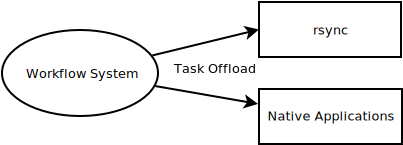
\includegraphics[scale=0.45]{figures/offload.pdf}
    \end{center}
    \caption{Performance: Task offload}
    \label{eval:offload}
\end{figure}

Due to this a performance evaluation of the system was not deemed necessary.
Performance of the system could however be affected by several processes being
executed simultaneously. In order to speed up the process in this regard the
system would need to be distributed to include multiple processing servers this
was unfortunately outside the scope of the project.


\chapter{Conclusion}
\section{Future Work}
During the implementation of the workflow system various possible extensions
that could be added to the system however due to constraints on time these could
not be implemented. These features would improve the system both in terms of
performance, usability and set up time.

\begin{description}
\item[Hierarchical Workflows]\hfill \\
To allow better control and reusability over tasks, workflows should be
abstracted to include a hierarchy. Such a hierarchy would allow entire workflows
to be represented as singular nodes. These workflows, could then be repackaged
and reused in different sites, or even the same site. This would also allow the
setup for new sites to be much faster as prepackaged workflows could easily be
used as drop in components.
\item[Parameterized Scripts]\hfill \\
Oftentimes particular parameters of a script can change from one site to
another. This change does not necessarily affect the \emph{Task type}, however
with the current implementation of the system the change would need to be made
at this point. This can be greatly improved by allowing a \emph{Task} to send
parameters to the job. This would require the Task Subsystem to allow parameters
dynamically be sent to the \emph{Task Type}.
\item[Rule Based File Filters]\hfill \\
Currently within the system all the files in the output directory of a task is
treated as input to successor tasks. Tasks often times only use a portion of the
files created by the predecessor. In order to currently facilitate this with the
system additional a filtering task would need to be set up that filters out
unused files. By including a rule based filtering system much greater control
can be placed on the output files. Such rule based filters have been
successfully implemented in other systems\cite{conery2005rule}.
\item[Interactive Task Feedback Options]\hfill \\
In order to avoid one of the problems that were found in Section~\ref{eval:simple}
more interactivity is required for \emph{Tasks}. This primarily includes
real-time updates on the status of tasks. Further developments include the
ability to do more interactive validation such as discussion integration.
The addition of these collaborative could allow for a system that allows issues
with tasks for be resolved in a uniform manner\cite{guimaraes1998integration}.
\item[Transformation-based Task Support]\hfill \\
Currently the system is built around creating derivative data items. However it
is often common for certain files within a site to change, without creating an
additional copy. Although this behaviour is implicitly allowed it should be
extended to be better defined within the system.
\item[Parallel Task Processing] \hfill \\
One of the most crucial aspects affecting the long term feasibility of the
system is its ability to scale and handle larger and more complicated workflows.
In this regard the server node would become a significant bottleneck in
processing \emph{Server Tasks}. In order to alleviate this problem the system
would need to become distributed. This would present its own set of problems
as data would need to be efficiently distributed between the computation nodes
to ensure efficiency.

\end{description}

\bibliography{bibliography}{}
\bibliographystyle{apalike}
\appendix
\includepdf[pages=-,picturecommand*={%
     \put(42,760){%
              \parbox{\textwidth}{\chapter{Questionnaire}\label{appendix:questionnaire}}
	      }}]{survey.pdf}


\end{document}
